\section{Diseños de la aplicación}

El diseño de la interfaz es uno de los grandes retos del proyecto. Desde una posición más técnica y funcional realizar un diseño correcto era un trabajo difícil. Principalmente utilicé las técnicas de diseño presentadas en \cite{refactoring-ui}.

\subsection{Moodboard}

Antes de comenzar a realizar diseños, tenía que decidir los estilos a seguir. En primer lugar, estuve considerando el tipo de letra mayoritaria de la aplicación. Normalmente, se suele atribuir a los tipos de letra de tipo serif un ``look'' más clásico o elegante, para diseños que quieran transmitir seguridad y elegancia. Por otra parte, para diseños mas informales o cercanos se suelen utilizar tipos de letra sans-serif \cite[p.~21]{refactoring-ui}. En mi caso decidí utilizar tipos de letra sans-serif, ya que no era necesario transmitir seguridad o confianza, algo más propio de entidades como bancos o seguros. En mi caso me decanté por la tipografía OpenSans en todas sus variantes, la que al ser libre, me permitiría utilizarla respetando sus licencias sin cargos extra para la fundación.

\begin{figure}[h!]
    \centering
    
\includegraphics[width=0.9\linewidth]{diseno/app/presentacion/opensans.png}
\end{figure}

\begin{wrapfigure}{r}{0.35\textwidth}
    \centering
    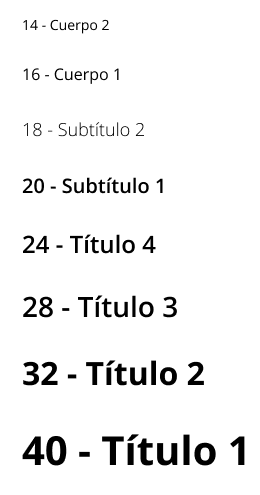
\includegraphics[width=0.9\linewidth]{diseno/app/presentacion/tamano.png}
\end{wrapfigure}

Una vez seleccionada la fuente principal a utilizar, tenía que decidir los tamaños a utilizar. Siguiendo los guidelines de tipografías tanto de IOS \cite{typ-ios} como de Material Design \cite{typ-android}, utilicé una fuente de letra mínima de 14px para cuerpos de texto grandes y una máxima de 40 px para títulos. Junto con esto, utilicé tres variaciones de la fuente de letra para hacer más énfasis y diferenciar los textos más importantes. 

Para los tamaños de los iconos utilicé el mismo sistema, siguiendo del mismo modo ambas guidelines. El pack de iconos utilizado en todos los diseños es \href{https://heroicons.com/}{Heroicons}, desarrollado por \href{https://github.com/tailwindlabs}{Tailwind Labs} bajo una licencia MIT.

Para el color elegí utilizar solo uno como color principal y basar el diseño en las diferentes sombras de grises de este. Esto simplificó el proceso de diseño. Escogí un tono cyan como color principal (\textit{\#086d80} 
\includegraphics[height=\fontcharht\font`\B]{diseno/app/presentacion/color.png}) y un tono amarillo para alertas y avisos (\textit{\#ffd98f} 
\includegraphics[height=\fontcharht\font`\B]{diseno/app/presentacion/amarillo.png})

\subsection{Diseños}

En una primera versión de los diseños estos fueron desarrollados en escala de grises obviando los colores elegidos previamente. Realizarlos de esta forma permitiría elegir mejor los márgenes a utilizar, contraste entre elementos y tamaños \cite[p.~13]{refactoring-ui}. 

\begin{figure}[h!]
    \centering
    
    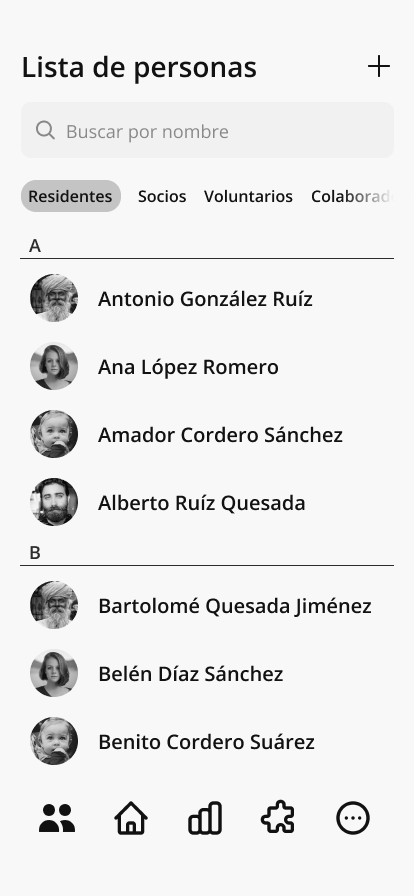
\includegraphics[width=0.30\linewidth]{diseno/app/bw/Principal personas.png}
    \hspace{0.03\linewidth}
    \includegraphics[width=0.30\linewidth]{diseno/app/bw/Al pulsar en añadir cita.png}
    \hspace{0.03\linewidth}
    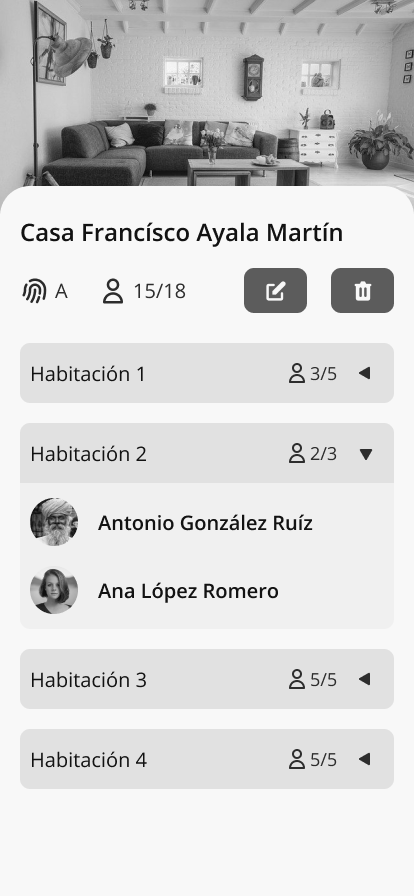
\includegraphics[width=0.30\linewidth]{diseno/app/bw/Datos de una casa.png}

    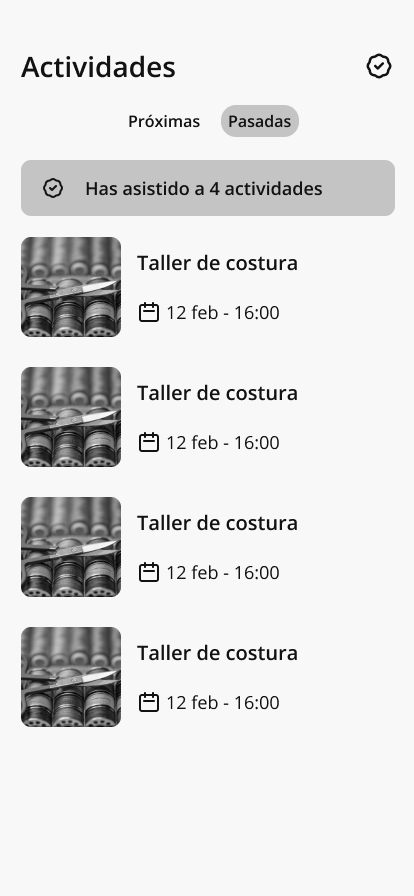
\includegraphics[width=0.30\linewidth]{diseno/app/bw/Principal actividades asistente.png}
    \hspace{0.03\linewidth}
    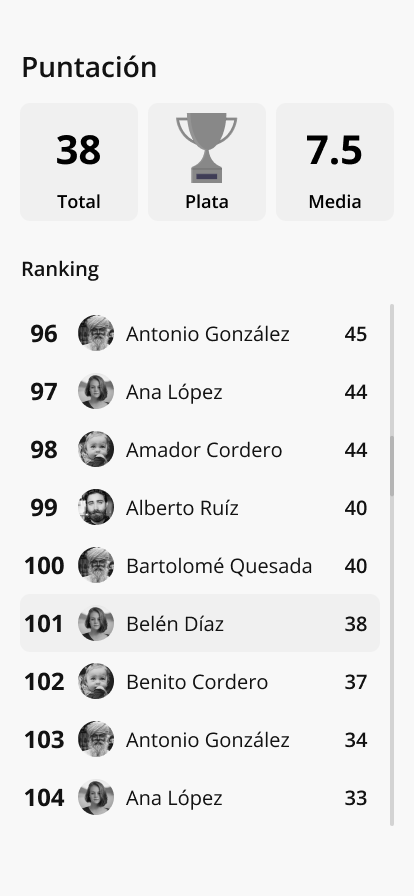
\includegraphics[width=0.30\linewidth]{diseno/app/bw/Ranking.png}
    \hspace{0.03\linewidth}
    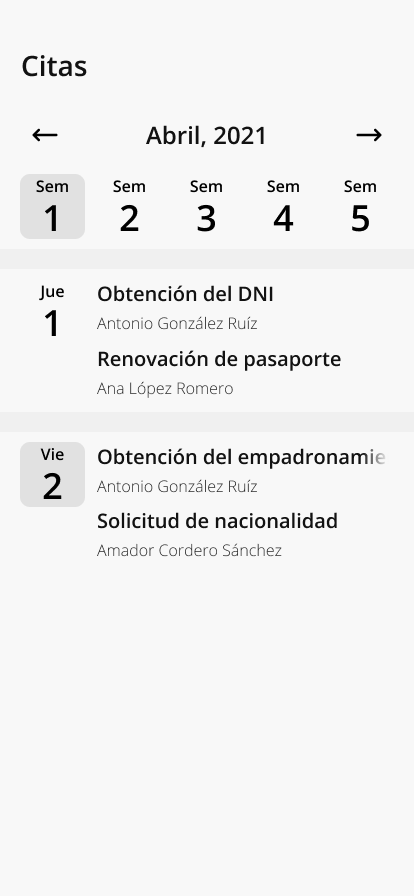
\includegraphics[width=0.30\linewidth]{diseno/app/bw/Citas.png}

    \caption{Primera versión de los diseños}
    \label{fig:dis-bw}

\end{figure}

Una vez basándome en estos diseños y en los estilos especificados en el Moodboard, se completó este añadiendo colores, detalles, así como otras pantallas interesantes.

\begin{figure}[h!]
    % \centering
    \minipage{0.30\textwidth}
        % \centering
        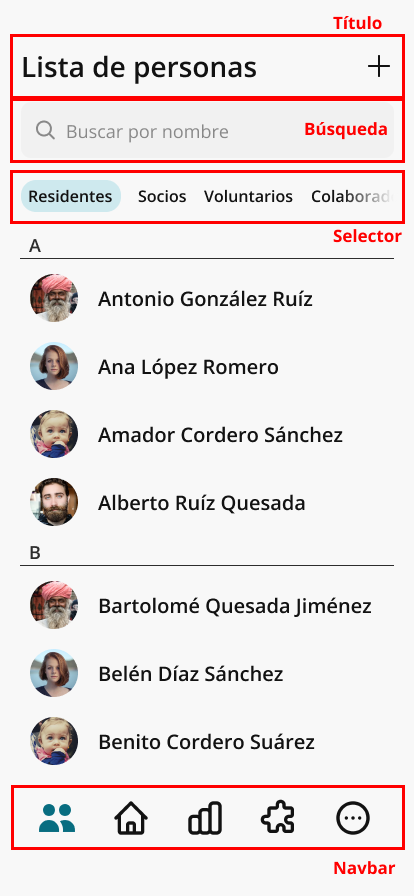
\includegraphics[width=\linewidth]{diseno/app/presentacion/secciones.png}
    \endminipage\hfill
    \minipage{0.30\textwidth}
        \centering
        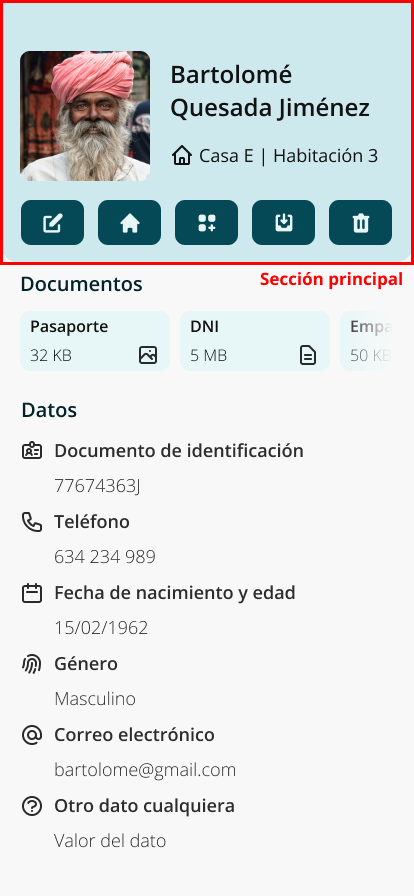
\includegraphics[width=\linewidth]{diseno/app/presentacion/secciones-elemento.png}
    \endminipage\hfill
    \minipage{0.30\textwidth}
        \centering
        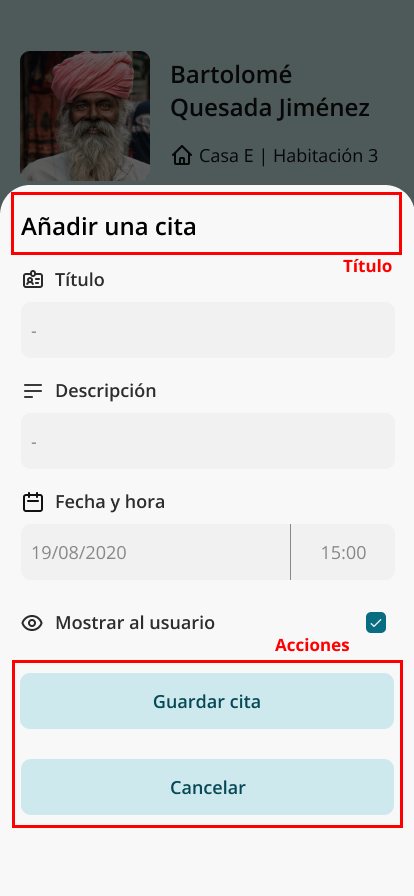
\includegraphics[width=\linewidth]{diseno/app/presentacion/secciones-popup.png}
    \endminipage
    \caption{ Secciones de comunes en las pantallas. De izquierda a derecha: página principal, pantalla de un elemento, pantalla de popup }
    \label{fig:secciones}
\end{figure}

Muchos de las pantallas comparten componentes, lo que hace que la aplicación parta de varios diseños únicos y que a partir de ahí cada pantalla añada sus propio contenido. Todas las pantallas principales (como la que se ve en la Figura \ref{fig:secciones} (izquierda)) tendrán un \textit{barra de navegación} inferior en la que se podrá navegar a través de las diferentes secciones de la app. Por otra parte, otro componente que compartirán muchas pantallas será el título. Este ofrecerá información acerca de la pantalla que se visita, así como una acción opcional a realizar. Por otra parte, según la pantalla podrían aparecer selectores de contenido así como una barra de búsqueda. El espacio restante lo ocupará el contenido.      

Por otra parte, en pantallas que representan a un elemento en específico (como la que se ve en la Figura \ref{fig:secciones} (centro)) ya sea un alojamiento, actividad o personas, el diseño cambiará. Se perderá la barra de navegación inferior, a la cual se podrá acceder volviendo a la pantalla anterior. La página en este caso se dividirá en una sección superior que nos aportará información acerca del elemento con el que estamos tratando, además de incluir acciones principales mediante botones. El resto de la pantalla será contenido asociado al elemento.

En tercer lugar, otra tipo de ``pantalla'' aparecerá como un ``popup'' (como se ve en la Figura \ref{fig:secciones} (derecha)) para confirmar o realizar alguna una acción. Este se dividirá en tres partes, el título, el contenido y los botones de acción.

Los diseños finales de algunas de las pantallas son los mostrados en las figuras \ref{fig:dis-fin1} y \ref{fig:dis-fin2}.

\begin{figure}[hp!]
    \centering
    
    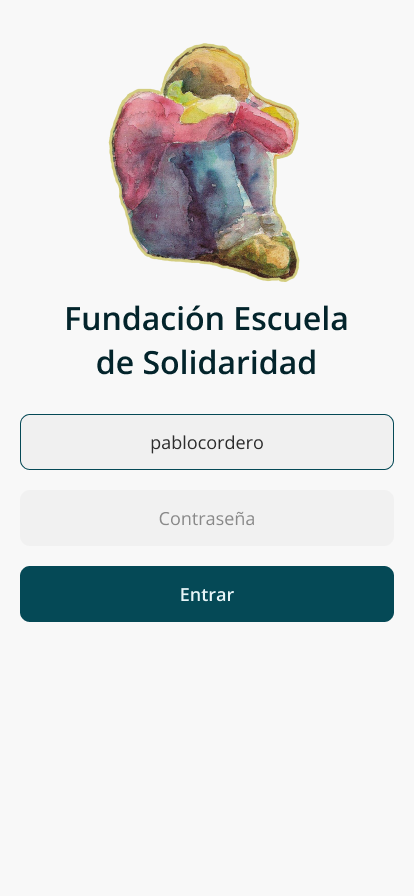
\includegraphics[width=0.30\linewidth]{diseno/app/Login.png}
    \hspace{0.03\linewidth}
    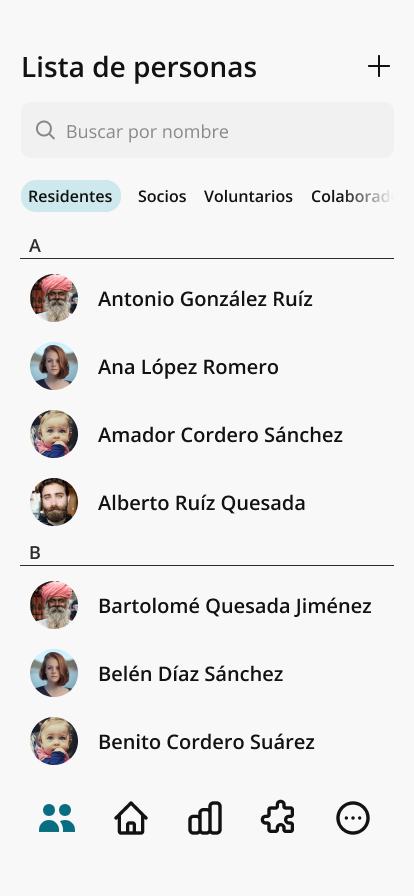
\includegraphics[width=0.30\linewidth]{diseno/app/Principal personas.png}
    \hspace{0.03\linewidth}
    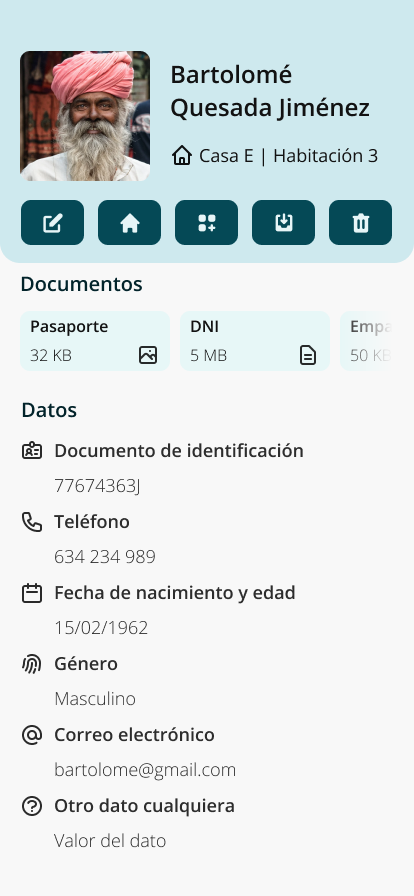
\includegraphics[width=0.30\linewidth]{diseno/app/Datos de persona.png}

    \includegraphics[width=0.30\linewidth]{diseno/app/Añadir una persona.png}
    \hspace{0.03\linewidth}
    \includegraphics[width=0.30\linewidth]{diseno/app/Al pulsar en añadir cita.png}
    \hspace{0.03\linewidth}
    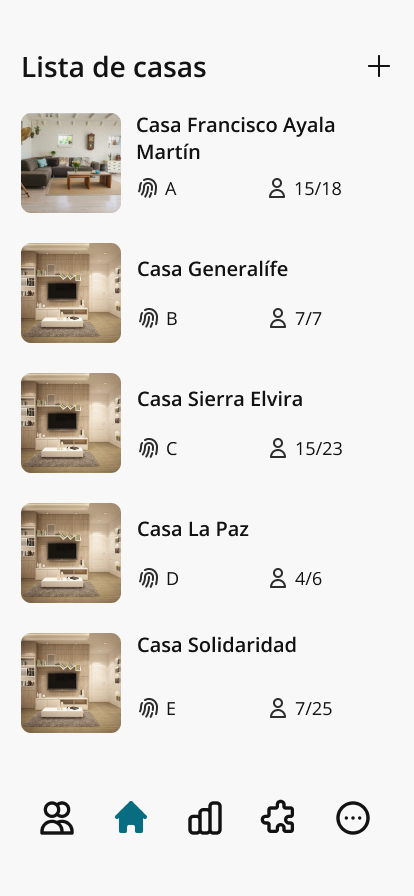
\includegraphics[width=0.30\linewidth]{diseno/app/Principal casas.png}

    \caption{Versión final de los diseños (1)}
    \label{fig:dis-fin1}

\end{figure}

\begin{figure}[hp!]
    \centering
    
    \includegraphics[width=0.30\linewidth]{diseno/app/Principal estadísticas.png}
    \hspace{0.03\linewidth}
    \includegraphics[width=0.30\linewidth]{diseno/app/Editar una habitación.png}
    \hspace{0.03\linewidth}
    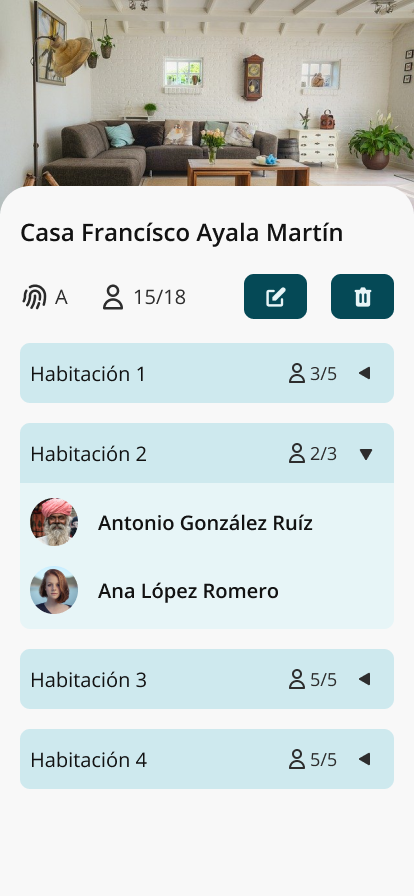
\includegraphics[width=0.30\linewidth]{diseno/app/Datos de una casa.png}

    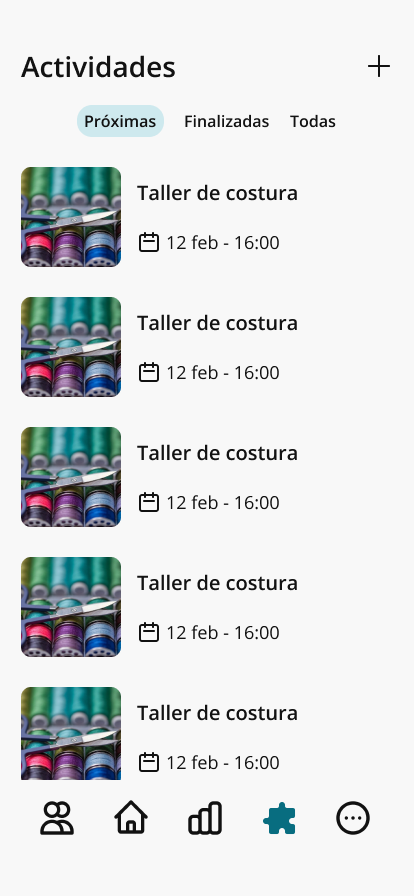
\includegraphics[width=0.30\linewidth]{diseno/app/Principal actividades admin.png}
    \hspace{0.03\linewidth}
    \includegraphics[width=0.30\linewidth]{diseno/app/Visión de una actividad.png}
    \hspace{0.03\linewidth}
    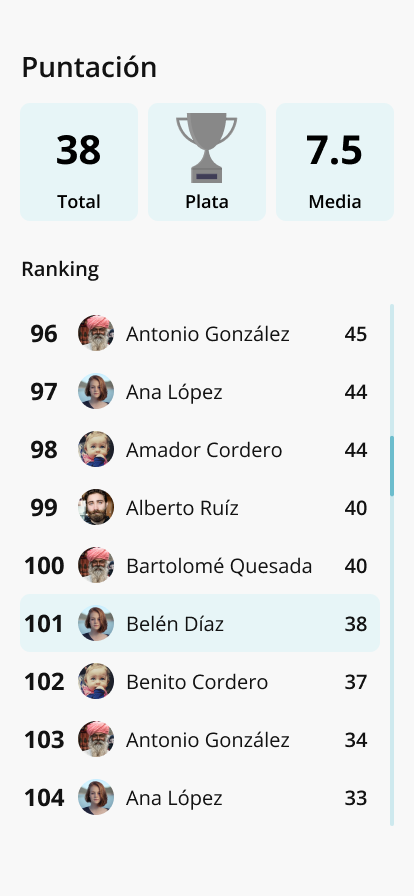
\includegraphics[width=0.30\linewidth]{diseno/app/Ranking.png}

    \caption{Versión final de los diseños (2)}
    \label{fig:dis-fin2}

\end{figure}

\newpage

A todo esto se le incluye un diseño de ``workflow'' el cual permitirá entender mejor los diseños comprendiendo qué acciones se pueden realizar y como se navegaría a través de la aplicación

\begin{figure}[h!]
    \centering
    \includegraphics[width=\linewidth]{diseno/app/presentacion/workflow.png}
\end{figure}
